\documentclass{article}
\usepackage[utf8]{inputenc}
\usepackage{ gensymb }
\usepackage{ dsfont }
\usepackage{polski}
\usepackage{ textcomp }
\usepackage{amsmath}
\usepackage{ wasysym }
\usepackage{graphicx}
\usepackage{ amssymb }

\setlength{\textheight}{24cm}
\setlength{\textwidth}{15.92cm}
\setlength{\footskip}{10mm}
\setlength{\oddsidemargin}{0mm}
\setlength{\evensidemargin}{0mm}
\setlength{\topmargin}{0mm}
\setlength{\headsep}{5mm}

\title{Group and Ring Theory Problems in Polish}
\author{Andrzej "Mathinity" Kukla}
\date{ }

\usepackage{natbib}
\usepackage{graphicx}
\usepackage{ dsfont }

\begin{document}

\maketitle
\begin{center}
\Large \textbf{1.} $X=\{1...n\}$ i $A_n:=\{ \sigma :X \rightarrow X \ |\  \sigma \ bijekcja \wedge sgn(\sigma) = 1\}$

Niech $B_n=\{(i_1 i_2 i_3): i_j \in X\ dla\ j\in \{1,2,3\}\}$ T:$\langle B_n\rangle=A_n$
\end{center}
\normalsize

Dw. 

Niech $A\in A_n$. Wtedy A to złożenie $k$ cykli różnych długości, które zawierają w sobie w sumie $r$ elementów X. Wtedy: $sgn(A)=(-1)^{n-(k+(n-r))}=(-1)^{r-k}$. Aby $sgn(A)=1$, to $r-k$ musi być liczbą parzystą.

$1^{\degree }$ $r$ nieparzyste $\Rightarrow$ $k$ nieparzyste.

Wtedy liczba cykli o parzystej liczbie el. musi być parzysta, a liczba cykli o nieparzystej liczbie el. musi być nieparzysta. Każdy z cykli da się rozłożyć na iloczyn transpozycji. Każdy cykl o parzystej liczbie el. rozłoży się na iloczyn nieparzystej liczby transpozycji, a każdy cykl o nieparzystej liczbie el. rozłoży się na iloczyn parzystej liczby transpozycji. Ostatecznie dostajemy iloczyn parzystej liczby transpozycji. Transpozycje możemy przekształcić w 3-cykle w następujący sposób: 

Niech $a,b,c,d\in X$ są parami rozłączne. Wtedy:
\begin{eqnarray}
(ab)(ac)&=&(acb)\\
(ab)(cd)&=&(bcd)(adb)
\end{eqnarray}


Cykle o nieparzystej liczbie el. rozkładają się iloczyn 3-cykli jedynie typu (1), natomiast cykle o parzystej liczbie el. rozkładają się na iloczyn 3-cykli typu (1) i (2). Liczba cykli o parzystej liczbie el. jest nieparzysta, więc rozłożą się one na iloczyn jedynie 3-cykli (2 takie cykle wyprodukują 1 3-cykl typu (2)).

Z tego wynika, że $A\in <B_n>$ 

$2^{\degree }$ $r$ parzyste $\Rightarrow$ $k$ parzyste.

Wtedy iloczyn składa się z parzystej liczby cykli o parzystej liczbie el. i parzystej liczbie cykli o nieparzystej liczbie el. Rozkładając te cykle na iloczyn transpozycji dostajemy ich parzystą ilość, więc możemy je złożyć w 3-cykle. Stąd $A\in \langle B_n\rangle$ 
\begin{flushright}
$\blacksquare$
\end{flushright}

\begin{center}
\Large{\textbf{2.} Znaleźć wszystkie podgrupy grupy $D_6$}
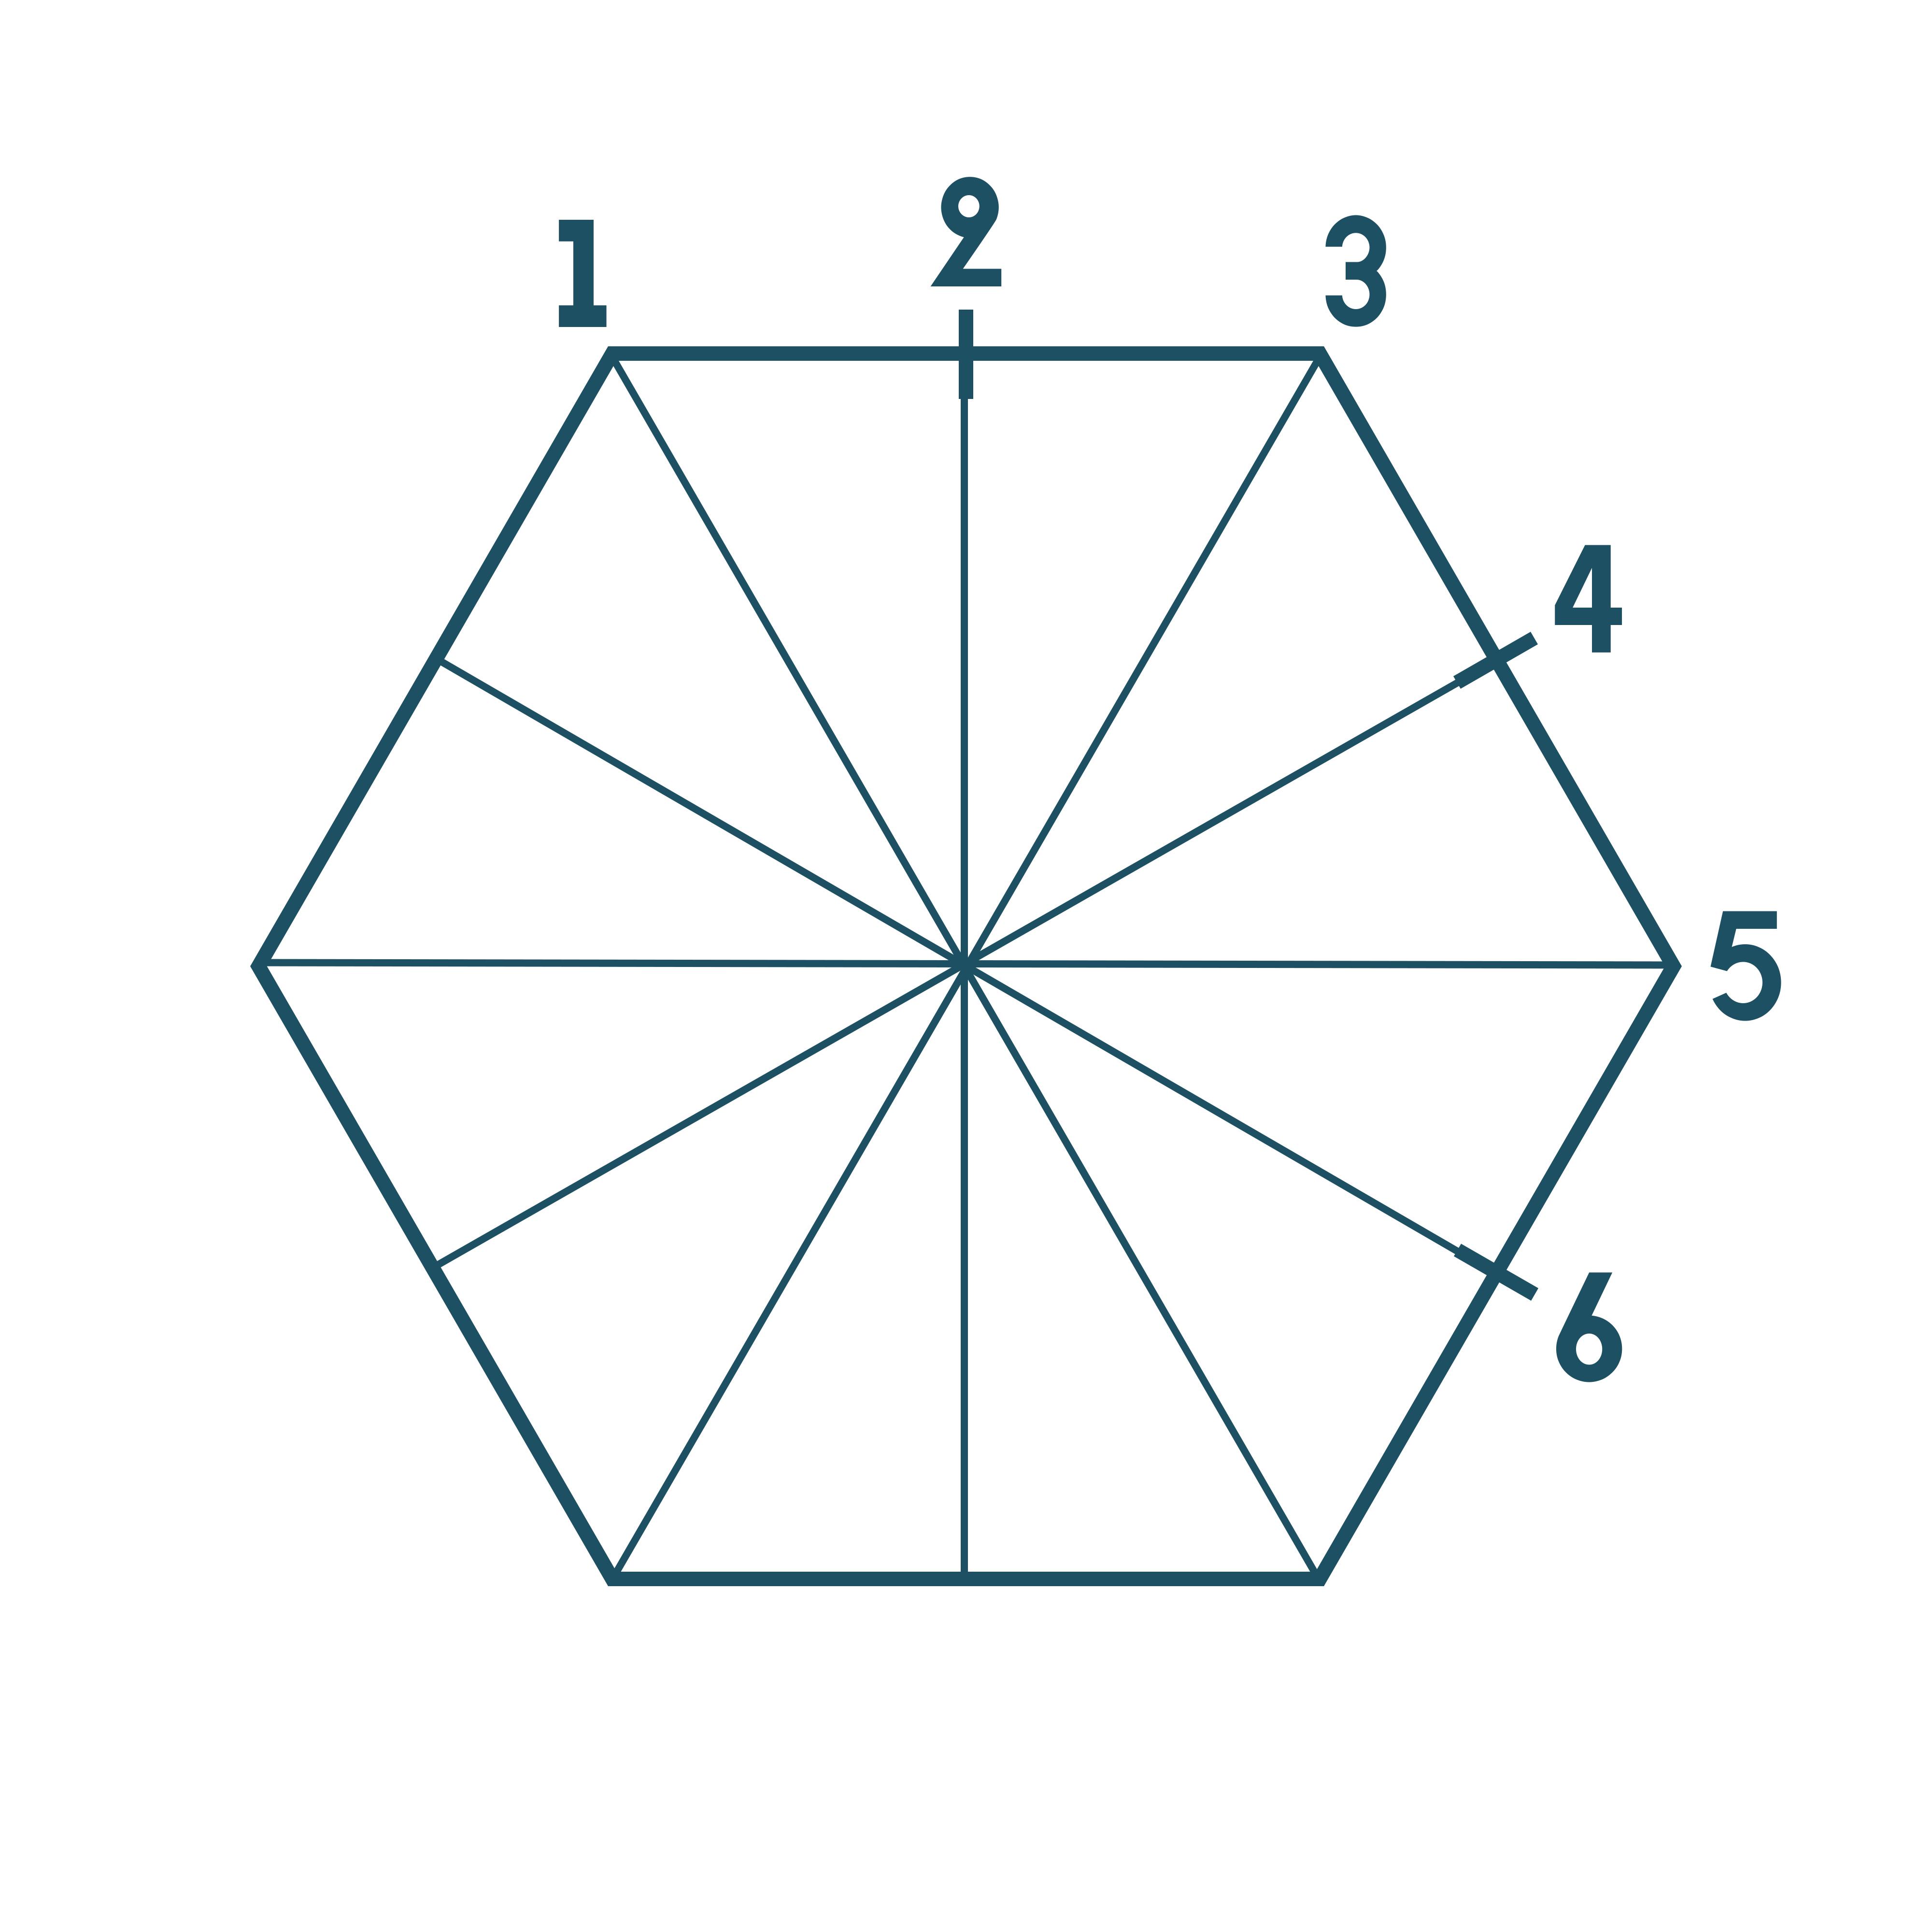
\includegraphics[scale=0.07]{sześciokąt foremny.jpg}
\end{center}
Niech 

- $s(i)$ to symetria względem symetralnej wychodzącej z punktu oznaczonego na rysunku, $i\in \{1,...,6\}$;

- $o(x)$ to obrót o x-kąt, zgodny z ruchem wskazówek zegara, $x\in (0,2\pi)$;

Wtedy $D_6=\{id, s(1), s(2), s(3), s(4), s(5), s(6), o(\frac{\pi}{3}), o(\frac{2\pi}{3}), o(\pi), o\left(\frac{4\pi}{3}\right), o\left(\frac{5\pi}{3}\right)\}$

Kilka obserwacji: 

$$\forall i\in \{1,...,6\}: s(i)^{-1}=s(i)$$
$$\forall x\in (0,2\pi): o\left(\frac{x\pi}{3}\right)^{-1}=o\left(\frac{(6-x)\pi}{3}\right)$$

Podgrupy oczywiste: 
\begin{itemize}
    \item $H_1=\{id\}$
    \item $H_2=D_6$
    \item $H_3=\{id, s(1)\}$
    \item $H_4=\{id, s(2)\}$
    \item $H_5=\{id, s(3)\}$
    \item $H_6=\{id, s(4)\}$
    \item $H_7=\{id, s(5)\}$
    \item $H_8=\{id, s(6)\}$
    \item $H_9=\{id, o(\frac{\pi}{3}), o(\frac{5\pi}{3})\}$
    \item $H_{10}=\{id, o(\frac{2\pi}{3}), o(\frac{4\pi}{3})\}$
    \item $H_{11}=\{id, o(\pi)\}$
\end{itemize}

Jeżeli stworzymy grupę $H=\{id,o(\frac{x\pi}{3}),o(\frac{y\pi}{3})\}$, gdzie $x,y\in (0,2\pi)$ i $x\neq y$, to jesteśmy zmuszeni dodać do niej odwrotności $o(\frac{x\pi}{3})$ i $o(\frac{y\pi}{3})$, a jak się okazuje także wszystkie pozostałe obroty z $D_6$. 

Zatem $H_{11}=\{id, o(\frac{\pi}{3}), o(\frac{2\pi}{3}), o(\pi), o(\frac{4\pi}{3}), o(\frac{5\pi}{3})\}$.

Jeżeli stworzymy grupę $H=\{id, s(i), s(j)\}$, gdzie $i,j\in \{1,...,6\}$ i $i\neq j$, to jesteśmy zmuszeni dodać do niej obrót, który jest złożeniem tych dwóch symetrii, a co za tym idzie musimy dodać złożenia symetrii i obrotów. Oto zestawienie wszystkich złożeń obrotów i symetrii:



\begin{center}
(najpierw kolumna, potem wiersz)

\ 

\begin{tabular}{c|c c c c c}
$\circ$  & $o(\frac{\pi}{3})$ & $o(\frac{2\pi}{3})$ & $o(\pi)$ & $o(\frac{4\pi}{3})$ & $o(\frac{5\pi}{3})$ \\\hline
$s(1)$ & $s(6)$ & $s(5)$ & $s(4)$ & $s(3)$ & $s(2)$  \\
$s(2)$ & $s(1)$ & $s(6)$ & $s(5)$ & $s(4)$ & $s(3)$  \\
$s(3)$ & $s(2)$ & $s(1)$ & $s(6)$ & $s(5)$ & $s(4)$  \\
$s(4)$ & $s(3)$ & $s(2)$ & $s(1)$ & $s(6)$ & $s(5)$  \\
$s(5)$ & $s(4)$ & $s(3)$ & $s(2)$ & $s(1)$ & $s(6)$  \\
$s(6)$ & $s(5)$ & $s(4)$ & $s(3)$ & $s(2)$ & $s(1)$ 
\end{tabular}

\ 

(najpierw wiersz, potem kolumna)

\ 

\begin{tabular}{c|c c c c c}


$\circ$  & $o(\frac{\pi}{3})$ & $o(\frac{2\pi}{3})$ & $o(\pi)$ & $o(\frac{4\pi}{3})$ & $o(\frac{5\pi}{3})$ \\\hline
$s(1)$ & $s(2)$ & $s(3)$ & $s(4)$ & $s(5)$ & $s(6)$  \\
$s(2)$ & $s(3)$ & $s(4)$ & $s(5)$ & $s(6)$ & $s(1)$  \\
$s(3)$ & $s(4)$ & $s(5)$ & $s(6)$ & $s(1)$ & $s(2)$  \\
$s(4)$ & $s(5)$ & $s(6)$ & $s(1)$ & $s(2)$ & $s(3)$  \\
$s(5)$ & $s(6)$ & $s(1)$ & $s(2)$ & $s(3)$ & $s(4)$  \\
$s(6)$ & $s(1)$ & $s(2)$ & $s(3)$ & $s(4)$ & $s(5)$ 
\end{tabular}
\end{center}
Oto zestawienie wszystkich złożeń symetrii:
\begin{center}


(najpierw kolumna, potem wiersz)

\ 

\begin{tabular}{c|c c c c c c}
$\circ$ & $s(1)$ & $s(2)$ & $s(3)$ & $s(4)$ & $s(5)$ & $s(6)$ \\\hline
$s(1)$ & id & $o(\frac{5\pi}{3})$ & $o(\frac{4\pi}{3})$ & $o(\pi)$ & $o(\frac{2\pi}{3})$ &  $o(\frac{\pi}{3})$\\
$s(2)$ & $o(\frac{\pi}{3})$ & id & $o(\frac{5\pi}{3})$ &  $o(\frac{4\pi}{3})$ & $o(\pi)$ & $o(\frac{2\pi}{3})$\\
$s(3)$ & $o(\frac{2\pi}{3})$ & $o(\frac{\pi}{3})$ & id & $o(\frac{5\pi}{3})$ & $o(\frac{4\pi}{3})$ & $o(\pi)$\\
$s(4)$ & $o(\pi)$ & $o(\frac{2\pi}{3})$ & $o(\frac{\pi}{3})$ & id & $o(\frac{5\pi}{3})$  & $o(\frac{4\pi}{3})$\\
$s(5)$ & $o(\frac{4\pi}{3})$ & $o(\pi)$ & $o(\frac{2\pi}{3})$ & $o(\frac{\pi}{3})$ & id &$o(\frac{5\pi}{3})$ \\
$s(6)$ & $o(\frac{5\pi}{3})$ & $o(\frac{4\pi}{3})$ & $o(\pi)$ & $o(\frac{2\pi}{3})$ & $o(\frac{\pi}{3})$ & id 
\end{tabular}

\end{center}

Można zauważyć, że dla różnych par symetrii utworzą się różne podgrupy. Mamy:

- $s(1)\circ s(2)$, $s(1)\circ s(6)$, $s(2)\circ s(3)$, $s(3)\circ s(4)$, $s(4)\circ s(5)$ i $s(5)\circ s(6)$ 

generują $D_6$

- $s(1)\circ s(3)$, $s(1)\circ s(5)$ i $s(3)\circ s(5)$ 

generują $H_{12}=\{id,s(1),s(3),s(5), o(\frac{2\pi}{3}),o(\frac{4\pi}{3})\}$

- $s(2)\circ s(4)$, $s(2)\circ s(6)$ i $s(4)\circ s(6)$

generują $H_{13}=\{id,s(2),s(4),s(6), o(\frac{2\pi}{3}),o(\frac{4\pi}{3})\}$

- $s(1)\circ s(4)$ 

generuje $H_{14}=\{id,s(1),s(4),o(\pi)\}$

- $s(2)\circ s(5)$ 

generuje $H_{15}=\{id,s(2),s(5),o(\pi)\}$

- $s(3)\circ s(6)$ 

generuje $H_{16}=\{id,s(3),s(6),o(\pi)\}$.

\ 
\begin{center}
 \Large \textbf{3.} Znaleźć wszystkie izomorfizmy $\mathds{Z}/12 \rightarrow \mathds{Z}/12$
  
\end{center}

Niech $f(x): \mathds{Z}/12 \rightarrow \mathds{Z}/12$ będzie izomorfizmem. Wtedy: $\forall a,b\in \mathds{Z}/12$: $f(a+b)=f(a)+f(b)$.

1) Niech $b=a$.

Wtedy $f(2a)=2f(a)\Rightarrow f(0)=0\wedge f(6)=6$.

2) Niech $b=-a$ w sensie $mod12$.

Wtedy $f(0)=f(a)+f(-a)\Rightarrow -f(-a)=f(a)$.

3) Niech $a=1$. 

Wtedy: $f(2)=f(1)-f(11)$.

\ 

Podstawiając za $f(1)$ kolejne elementy zbioru $\mathds{Z}/12$ uzyskujemy sprzeczność dla $$f(1)\in \{0,2,3,4,6,8,9,10\}$$ 

Gdy podstawimy $f_1(1)=1$ uzyskujemy identyczność.

Gdy podstawimy $f_2(1)=5$ uzyskujemy następujący izomorfizm:
\begin{center}
\begin{tabular}{c|c c c c c c c c c c c c}
x & 0 & 1 & 2 & 3 & 4 & 5 & 6 & 7 & 8 & 9 & 10 & 11 \\\hline
f(x) & 0 & 5 & 10 & 3 & 8 & 1 & 6 & 11 & 4 & 9 & 2 & 7 \\
\end{tabular}
\end{center}

Gdy podstawimy $f_3(1)=7$ uzyskujemy następujący izomorfizm:
\begin{center}
\begin{tabular}{c|c c c c c c c c c c c c}
x & 0 & 1 & 2 & 3 & 4 & 5 & 6 & 7 & 8 & 9 & 10 & 11 \\\hline
f(x) & 0 & 7 & 2 & 9 & 4 & 11 & 6 & 1 & 8 & 3 & 10 & 5 \\
\end{tabular}
\end{center}

Gdy podstawimy $f_4(1)=11$ uzyskujemy następujący izomorfizm: 
$f(x) = -x$

Zbiór powyższych izomorfizmów $Izom$ z działaniem $\circ:Izom\times Izom\rightarrow Izom$ tworzą monoid, ponieważ $\circ$ jest działaniem łącznym oraz el. neutralny: $id=f_1(x)$ należy do $Izom$, ale nie jest to grupa, ponieważ nie istnieje element odwrotny np. do $f_2(x)$.

\begin{center}
\Large{\textbf{4.} Pokazać, że w $S_4$ jedyną podgrupą rzędu 12 jest $A_4$. }
\end{center}
\normalsize{}
\begin{center}
\textbf{Hp.} $\exists H<S_4:|H|=12 \wedge H\neq A_4$
\end{center}
Z tw. Lagrange'a wiemy, że $|S_4|=|H|\ |S_4:H| \Rightarrow |S_4:H|=2$. Stąd wiemy, że podgrupa $H$ jest normalna oraz grupa $S_4/H $ jest abelowa. W szczególności $S_4'<H$.

Z tego samego powodu co powyżej wiemy, że $S_4'<A_4$. Pokażę teraz, że $S_4'>A_4$. Istotnie weźmy dowolny 3-cykl $(ijk)\in S_4$. Mamy:
\begin{align*}
    (ijk)& =(ikj)^2=((ik)(ij))^2=(ik)(ij)(ik)(ij)=\\
    & =(ik)(ij)(ik)^{-1}(ij)^{-1}=[(ik),(ij)]\in S_4'
\end{align*}
Jako że podgrupa $A_4$ jest generowana przez 3-cykle, to $S_4'>A_4$. 

Z powyższego rozumowania wynika, że $S_4'=A_4$, więc w szczególności $A_4<H$, ale $|A_4|=|H|$, więc $A_4=H$ - sprzeczność.
\begin{flushright}
$\blacksquare$
\end{flushright}

\begin{center}
\Large \textbf{5.} Ile jest różnych grup abelowych rzędu $864$?
\end{center}
\normalsize{}

Niech $G$ grupa abelowa, $|G|=864=2^5\cdot 3^3$. Grupę G można przedstawić jako sumę prostą grup cyklicznych. Sprawdźmy wszystkie możliwości sum prostych (przedstawicielami grup będą ich rzędy):
\begin{center}
Suma prosta \textbf{dwóch} grup cyklicznych:
$$\#\{2^5\oplus3^3\}=1$$

Suma prosta \textbf{trzech} grup cyklicznych:
$$\#\{2\oplus2^4\oplus3^3,\quad2^2\oplus2^3\oplus3^3,\quad2^5\oplus3\oplus3^2\}=3$$

Suma prosta \textbf{czterech} grup cyklicznych:
$$\#\{2\oplus2\oplus2^3\oplus3^3,
\quad2\oplus2^2\oplus2^2\oplus3^3,
\quad2\oplus2^4\oplus3\oplus3^2,
\quad2^2\oplus2^3\oplus3\oplus3^2,
\quad2^5\oplus3\oplus3\oplus3\}=5$$


Suma prosta \textbf{pięciu} grup cyklicznych:
$$\#\{2\oplus2\oplus2\oplus2^2\oplus3^3,
\quad2\oplus2\oplus2^3\oplus3\oplus3^2,
\quad2\oplus2^2\oplus2^2\oplus3\oplus3^2,
\quad2\oplus2^4\oplus3\oplus3\oplus3,
\quad2^2\oplus2^3\oplus3\oplus3\oplus3
\}=5$$

Suma prosta \textbf{sześciu} grup cyklicznych:
$$\#\{2\oplus2\oplus2\oplus2\oplus2\oplus3^3,
\quad2\oplus2\oplus2\oplus2^2\oplus3\oplus3^2,
\quad2\oplus2^2\oplus2^2\oplus3\oplus3\oplus3,
\quad2\oplus2\oplus2^3\oplus3\oplus3\oplus3
\}=4$$

Suma prosta \textbf{siedmiu} grup cyklicznych:
$$\#\{2\oplus2\oplus2\oplus2\oplus2\oplus3\oplus3^2,
\quad2\oplus2\oplus2\oplus2^2\oplus3\oplus3\oplus3
\}=2$$

Suma prosta \textbf{ośmiu} grup cyklicznych:
$$\#\{2\oplus2\oplus2\oplus2\oplus2\oplus3\oplus3\oplus3
\}=1$$


Ostatecznie, grup abelowych rzędu $864$ jest $1+3+5+5+4+2+1=21$.
\end{center}

\begin{center}
\Large \textbf{6.} Skonstruować przykład nieabelowej grupy G rzędu 21 jako produkt półprosty $\mathds{Z}/7\rtimes \mathds{Z}/3$
\end{center}
Wiemy, że $\mathds{Z}/7=N\triangleleft G$ oraz $\mathds{Z}/3=Q<G$. Niech $\Theta:Q\ni q\rightarrow \Theta_q\in Aut(N)$. Wtedy $N\rtimes_\Theta Q=G$. Biorąc $\Theta_q=id$ dostaniemy grupę cykliczną rzędu 21, więc abelową. Tego nie chcemy. Weźmy: $$\Theta:Q\ni q\rightarrow2q\in \mathds{Z}/6\simeq Aut(N),$$ ponieważ jest to nietrywialny homomorfizm $\mathds{Z}/3\rightarrow\mathds{Z}/6 $. Jeśli $\varphi_0=id$ jest automorfizmem zadanym przez $1\rightarrow1$, $\varphi_1(1)=3$, to niech $\varphi_j=\varphi_1^j$. Wtedy $\varphi_2(1)=2,\quad\varphi_3(1)=6,\quad\varphi_4(1)=4,\quad\varphi_5(1)=5$. Widać, że $\varphi_1$ generuje $Aut(N)$ oraz $\varphi_j(1)=3^j mod7$, dla $j=0,...,5$.

Mamy zatem grupę $G=N\rtimes_\Theta=\mathds{Z}/7\rtimes\mathds{Z}/3$ z działaniem:
\begin{center}
$(a,x)(b,y)=(a+\Theta_x(b),x+y)=(a+\varphi_{2x}(b),x+y)=(a+3^{2x}b,x+y)$ mod 7 i mod 3.    
\end{center}

\begin{center}
\Large\textbf{7.} Sprawdzić, dla jakich $d\in\mathds{Z}$ (niebędących kwadratem) zbiór 
$$\mathds{Z}_{m}=\left\{a+b\frac{1+\sqrt{d}}{2}:a,b\in\mathds{Z}\right\}$$
z działaniami indukowanymi z $\mathds{R}$, jest pierścieniem.
\end{center}

Po pierwsze zauważmy, że dla każdego $d\in\mathds{Z}$ (niebędącego kwadratem) $(\mathds{Z}_m,+)$ jest grupą abelową. 

Niech $m=\frac{1+\sqrt{d}}{2}$. Oczywiście $m\in\mathds{Z}_m$. Pomnóżmy ze sobą dwa dowolne elementy $\mathds{Z}_m$ ($a,b,x,y\in\mathds{Z}$):

$$(a+bm)(x+ym)=ax+(ay+bx)m+bym^2$$

Sprawdźmy, kiedy $m^2\in\mathds{Z}_m$.

$$m^2=\left(\frac{1+\sqrt{d}}{2}\right)^2=\frac{1+2\sqrt{d}+d}{4}$$
\begin{flushleft}
$1\degree\quad d\equiv 0\mod4\Rightarrow m^2=\frac{d}{4}+\frac{1+2\sqrt{d}}{4}\Rightarrow m^2\notin\mathds{Z}_m$

$2\degree\quad d\equiv 1\mod4\Rightarrow m^2=\frac{d-1}{4}+\frac{2+2\sqrt{d}}{4}=\frac{d-1}{4}+\frac{1+\sqrt{d}}{2}\Rightarrow m^2\in\mathds{Z}_m$

$3\degree\quad d\equiv 2\mod4\Rightarrow m^2=\frac{d-2}{4}+\frac{3+2\sqrt{d}}{4}\Rightarrow m^2\notin\mathds{Z}_m$

$4\degree\quad d\equiv 3\mod4\Rightarrow m^2=\frac{d-3}{4}+\frac{4+2\sqrt{d}}{4}\Rightarrow m^2\notin\mathds{Z}_m$
\end{flushleft}

Widzimy, że jedyne $d\in\mathds{Z}$ niebędące kwadratem, dla którego $m^2\in\mathds{Z}_m$ to $$d\equiv1\mod4$$
Dla takiego d: $m^2=m+\frac{d-1}{4}$, dlatego też: $$m^3=m^2m=\left(m+\frac{d-1}{4}\right)m=m^2+\frac{d-1}{4}m=\frac{d-1}{4}+\left(\frac{d-1}{4}+1\right)m\in\mathds{Z}_m$$
Sprawdźmy, czy spełnione są pozostałe warunki:

$\cdot$ Czy dla dow. el. $a+bm$, $x+ym$, $p+qm\in\mathds{Z}_m$ mnożenie jest łączne?
$$((a+bm)(x+ym))(p+qm)=(ax+(ay+bx)m+bym^2)(p+qm)=$$
$$=axp+(ayp+bxp+axq)m+(byp+ayq+bxq)m^2+byqm^3=$$
$$=(a+bm)(xp+(xq+yp)m+yqm^2)=(a+bm)((x+ym)(p+qm))\ \checked$$

$\cdot$ Czy dla dow. el. $a+bm$, $x+ym$, $p+qm\in\mathds{Z}_m$ zachodzi rozdzielność mnożenia względem dodawania?
$$(a+bm+x+ym)(p+qm)=ap+xp+(bp+yp+aq+xq)m+(bq+yq)m^2$$
$$((a+bm)(p+qm))+((x+ym)(p+qm))=ap+(aq+bp)m+bqm^2+xp+(xq+yp)m+yqm^2\ \checked$$

\normalsize
$\cdot$ Czy istnieje element neutralny mnożenia?
$$1=1+0m\ \checked$$

\begin{center}
    \Large \textbf{(8a)} Znaleźć stopień rozszerzenia $\mathds{Q}(\sqrt[3]{2})$ nad $\mathds{Q}$
\end{center}

Na początek zauważmy, że $\sqrt[3]{2}$ jest algebraiczny nad $\mathds{Q}$, bo $x^3-2$ zeruje się dla $\sqrt[3]{2}$, więc $[\mathds{Q}(\sqrt[3]{2})/\mathds{Q}]\leq3$. Jako że $\sqrt[3]{2}\notin\mathds{Q}$ (istotnie, w równaniu $2a^3=b^3$ liczba dwójek w rozkładzie na liczby pierwsze w $2a^3$ zawsze przystaje do $1\mod3$, a w $b^3$ zawsze przystaje do $0\mod3$), to $[\mathds{Q}(\sqrt[3]{2})/\mathds{Q}]\geq2$.

Załóżmy, że bazą $\mathds{Q}(\sqrt[3]{2})$ nad $\mathds{Q}$ jest $1,\sqrt[3]{2}$. Sprawdźmy, czy $\sqrt[3]{4}\in\mathds{Q}(\sqrt[3]{2})$. Jeżeli tak, to
$$\sqrt[3]{4}=a+b\sqrt[3]{2}$$
po podniesieniu do sześcianu otrzymujemy
$$4=a^3+2b^3+3\sqrt[3]{2}a^2b+3\sqrt[3]{4}ab^2$$
ale bazą jest $1,\sqrt[3]{2}$, więc $3ab=0$, co daje sprzeczność. Wiemy jednak, że $$\sqrt[3]{2}^2=\sqrt[3]{4}\Rightarrow\sqrt[3]{4}\in\mathds{Q}(\sqrt[3]{2}),$$ więc $1,\sqrt[3]{2}$ nie może być bazą $\mathds{Q}(\sqrt[3]{2})$ nad $\mathds{Q}$. Stąd widać, że $[\mathds{Q}(\sqrt[3]{2})/\mathds{Q}]=3$.

\begin{center}
    \Large \textbf{(8b)} Znaleźć $a,b,c\in\mathds{Q}$ dla których
    $(1+\sqrt[3]{2}+\sqrt[3]{4})^{-1}=a+b\sqrt[3]{2}+c\sqrt[3]{4}$
\end{center}
$$(1+\sqrt[3]{2}+\sqrt[3]{4})(a+b\sqrt[3]{2}+c\sqrt[3]{4})=1$$
$$(a+2b+2c)+\sqrt[3]{2}(a+b+2c)+\sqrt[3]{4}(a+b+c)=1$$
Otrzymujemy układ równań:
$$\left\{\begin{array}{l}
a+2b+2c=1\\
a+b+2c=0\\
a+b+c=0
\end{array}\right.$$
z którego widać, że $a=-1, b=1, c=0$.
\end{document}